\documentclass[12pt]{article}

\usepackage[latin1]{inputenc}
\usepackage[T1]{fontenc}
\usepackage[francais]{babel}
%\usepackage{layout}
%\usepackage{geometry}
%\usepackage{setspace}
%\usepackage{soul}
%\usepackage{ulem}
%\usepackage{eurosym}
%\usepackage{bookman}
%\usepackage{charter}
%\usepackage{newcent}
%\usepackage{lmodern}
%\usepackage{mathpazo}
%\usepackage{mathptmx}
%\usepackage{url}
%\usepackage{verbatim}
%\usepackage{moreverb}
%\usepackage{listings}
%\usepackage{fancyhdr}
%\usepackage{wrapfig}
%\usepackage{color}
%\usepackage{colortbl}
\usepackage{amsmath}
\usepackage{amssymb}
\usepackage{mathrsfs}
\usepackage{amsthm}
%\usepackage{makeidx}
\usepackage{graphicx}
\usepackage{parskip}
\setlength{\parindent}{15pt}

\begin{document}

\title{ELEC1101: probl�me 1}
\author{Groupe 17}
\date{\today}
\maketitle

En lien avec le projet ELEC1101 de la majeure en �lectricit�, il a �t� demand� de s'int�resser aux s�ries de Fourier ainsi qu'aux transformations non linaires. Les diff�rentes questions pos�es � ce sujet constituent le premier probl�me autonome. Ce rapport tentera de donner r�ponse � celles-ci.

\section{Signal triangulaire et s�rie de Fourier}

Pour commencer, d�finissons un signal triangulaire quelconque comme repr�sent� sur la figure \ref{fig-trig}.

\begin{figure}[h]
\begin{center}
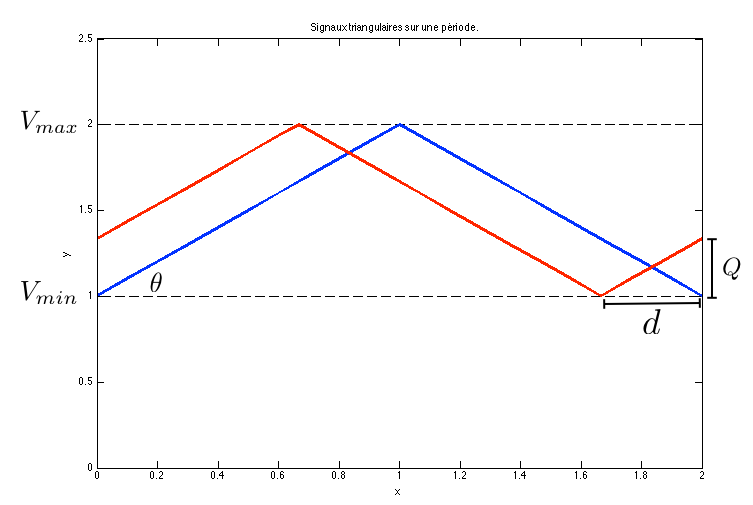
\includegraphics[width=\textwidth]{signal_triangulaire2}
\caption{Signaux triangulaires sur une p�riode}
\label{fig-trig}
\end{center}
\end{figure}

Un tel signal quelconque peut ici �tre s�parer en plusieurs segments de droites afin d'�tre d�crit de mani�re analytique. Int�ressons-nous pour ce faire au signal rouge, le plus g�n�ral des deux. Il peut �tre d�crit au moyen des �quation suivantes:
\begin{align}
d_{1}(t) = \tan(\theta)*t + V_{min} + Q\\
d_{2}(t) = -\tan(\theta)*t + V_{max} + Q - (V_{max}-V_{min})\\
d_{3}(t) = \tan(\theta)*t + V_{min} + Q - 2*(V_{max}-V_{min})
\label{}
\end{align}

\newpage
Dans ces expressions on peut lier certains param�tres entre eux et on obtient, avec T la p�riode:
$$\tan(\theta) = \frac{2*(V_{max}-V_{min})}{T}$$
$$d = \frac{Q}{\tan(\theta)}$$

Une fois ces expressions �tablies, il est possible d'obtenir le d�veloppement en s�rie de Fourier de ce signal. Pour ce faire il est n�cessaire de calculer les diff�rents coefficients de cette s�rie en s�parant le signal en 3 droites comme fait plus haut:
$$
\int_{0}^{T}{u(t) dt} =  \int_{0}^{\frac{T}{2}-d}{d_{1}(t) dt}+\int_{\frac{T}{2}-d}^{T-d}{d_{2}(t) dt}+\int_{T-d}^{T}{d_{3}(t) dt}
$$

En utilisant cette m�thode on obtient:
$$A_{0} = \frac{V_{max}+V_{min}}{2}$$
$$A_{k} = \frac{2*(V_{max}-V_{min})}{\pi^{2}k^{2}}*\left[\cos \left(k\pi \frac{Q-2(V_{max}-V_{min})}{V_{max}-V_{min}} \right) -  \cos \left(k\pi \frac{Q-(V_{max}-V_{min})}{V_{max}-V_{min}} \right)\right]$$

$$B_{k} = \frac{2*(V_{max}-V_{min})}{\pi^{2}k^{2}}*\left[\sin \left(k\pi \frac{Q-2(V_{max}-V_{min})}{V_{max}-V_{min}} \right) -  \sin \left(k\pi \frac{Q-(V_{max}-V_{min})}{V_{max}-V_{min}} \right)\right]$$

Le signal triangulaire $u(t)$ de pulsation $\omega$ peut donc enfin s'�crire:
\begin{align}
u(t) = A_{0} + \sum_{k=1}^{\infty}{A_{k}\cos(k\omega t)} + \sum_{k=1}^{\infty}{B_{k}\sin(k\omega t)} 
\label{serie-fourier}
\end{align}

Un choix judicieux de l'origine du temps permet de grandement simplifier ces expressions. En effet, placer le 0 sur un maximum ou un minimum du signal donne un signal pair. Le d�veloppement en s�rie de Fourier ne contient alors que des termes paires, c'est � dire le terme constant ainsi que la s�rie de cosinus. Avec les notations utilis�es plus haut, une telle situation correspond � $Q=0$ et les coefficients deviennent:
$$A_{0} = \frac{V_{max}+V_{min}}{2}$$
$$A_{k} = \frac{4*(V_{max}-V_{min})}{\pi^{2}(2k-1)^{2}}$$
$$B_{k} = 0$$




\end{document}
